\documentclass[11pt]{article}

\usepackage[a4paper]{geometry}
\geometry{left=2.0cm,right=2.0cm,top=2.5cm,bottom=2.5cm}


\usepackage{ctex} % 支持中文的LaTeX宏包
\usepackage{amsmath,amsfonts,graphicx,subfigure,amssymb,bm,amsthm,mathrsfs,mathtools,breqn} % 数学公式和符号的宏包集合
\usepackage{algorithm,algorithmicx} % 算法和伪代码的宏包
\usepackage[noend]{algpseudocode} % 算法和伪代码的宏包
\usepackage{fancyhdr} % 自定义页眉页脚的宏包
\usepackage[framemethod=TikZ]{mdframed} % 创建带边框的框架的宏包
\usepackage{fontspec} % 字体设置的宏包
\usepackage{adjustbox} % 调整盒子大小的宏包
\usepackage{fontsize} % 设置字体大小的宏包ddddddddd
\usepackage{tikz,xcolor} % 绘制图形和使用颜色的宏包
\usepackage{multicol} % 多栏排版的宏包
\usepackage{multirow} % 表格中合并单元格的宏包
\usepackage{pdfpages} % 插入PDF文件的宏包
\RequirePackage{listings} % 在文档中插入源代码的宏包
\RequirePackage{xcolor} % 定义和使用颜色的宏包
\usepackage{wrapfig} % 文字绕排图片的宏包

% ===== 代码样式自定义（lstlisting）=====
\definecolor{codegreen}{rgb}{0.0,0.5,0.0}
\definecolor{codegray}{rgb}{0.5,0.5,0.5}
\definecolor{codepurple}{rgb}{0.58,0,0.82}
\definecolor{codeblue}{rgb}{0.0,0.35,0.75}
\definecolor{codeorange}{rgb}{0.95,0.45,0.0}
\definecolor{codeback}{rgb}{0.96,0.96,0.97}
\lstset{
	language=Python,               % 默认语言
	basicstyle=\small\ttfamily,    % 基础字体
	keywordstyle=\color{codeblue}\bfseries,   % 关键字：蓝色加粗
	commentstyle=\color{codegreen}\itshape,   % 注释：绿色斜体
	stringstyle=\color{codepurple},           % 字符串：紫色
	numbers=left,                  % 左侧行号
	numberstyle=\tiny\color{codegray},
	numbersep=6pt,
	stepnumber=1,
	frame=single,                  % 单线边框
	framesep=5pt,
	rulecolor=\color{codegray},
	backgroundcolor=\color{codeback},   % 浅灰背景
	showstringspaces=false,
	breaklines=true,               % 自动换行
	breakatwhitespace=true,
	tabsize=4,
	columns=flexible,
	keepspaces=true,
	morekeywords={print,self,None,True,False}, % 额外高亮的关键字
}
\usepackage{bigstrut,multirow,rotating} % 支持在表格中使用特殊命令的宏包
\usepackage{booktabs} % 创建美观的表格的宏包
\usepackage{circuitikz} % 绘制电路图的宏包
\usepackage{makecell}
\graphicspath{{figure/}}

\usepackage{float} % 支持[H]浮动体定位
\newcommand{\blank}{\underline{\hspace{2.5em}}} % 留白占位，用于关键数据填写


\begin{document}
\begin{center}
	\LARGE \bf 液体厚度与颜色的深度学习
\end{center}
\section{实验目的}
\begin{enumerate}
	\item 观察并定量研究倾斜培养皿中液膜厚度的空间分布，理解厚度沿水平方向近似线性变化的规律；
	\item 依据 Beer-Lambert 定律，建立液膜厚度与颜色（吸光度、光强）之间的定量对应关系；
	\item 搭建“倾斜位移台—均匀漫射光源—相机”液膜测厚图像采集系统；
	\item 采集液膜厚度与颜色对应的图像数据集，训练深度学习模型（U-Net 等），实现由单幅相机图像反演液膜厚度分布；
	\item 检验标注与模型精度，验证基于颜色信息测量液体厚度的可行性与可靠性。
\end{enumerate}

\section{实验器材与用具}
\begin{itemize}
	\item 培养皿：透明玻璃（或光学级），平底；
	\item 去离子水、带色染料（预先标定浓度）；
	\item 可控体积转移工具：移液枪、量筒；
	\item 均匀白光光源：底部照明，光源上加纸片改造为漫反射光；
	\item X 轴角度倾斜平台（角度位移台，台面 $60\times60\,\mathrm{mm}$）、$100\times100\,\mathrm{mm}$ 光学转接板、M4 螺丝若干；
	\item 遮光黑布或暗箱（用于消除环境光）；
	\item 摄像系统：相机或手机，固定焦距及各项参数；
	\item 游标卡尺（测量培养皿深度、直径与底部厚度）。
\end{itemize}

\section{实验原理}
\subsection{液膜厚度与倾斜角的关系}
设培养皿内半径为 $R$、底部厚度为 $D$，注入体积为 $V$、浓度为 $c$ 的蓝色染液。培养皿水平放置时液深为
\[
	d = \frac{V}{\pi R^2}
\]
将培养皿绕水平轴倾斜角度 $\theta$ 后，液面仍保持水平，液膜形成楔形。以沿倾斜方向距培养皿中心 $x$ 处的液膜厚度记为 $h$，考虑到底面厚度 $D$ 的影响，有
\[
	h = (d+ D )\cos \theta  + R\sin\theta - x\tan\theta - \frac{D}{\cos \theta}
\]
如图所示：
\begin{figure}[H]
	\centering
	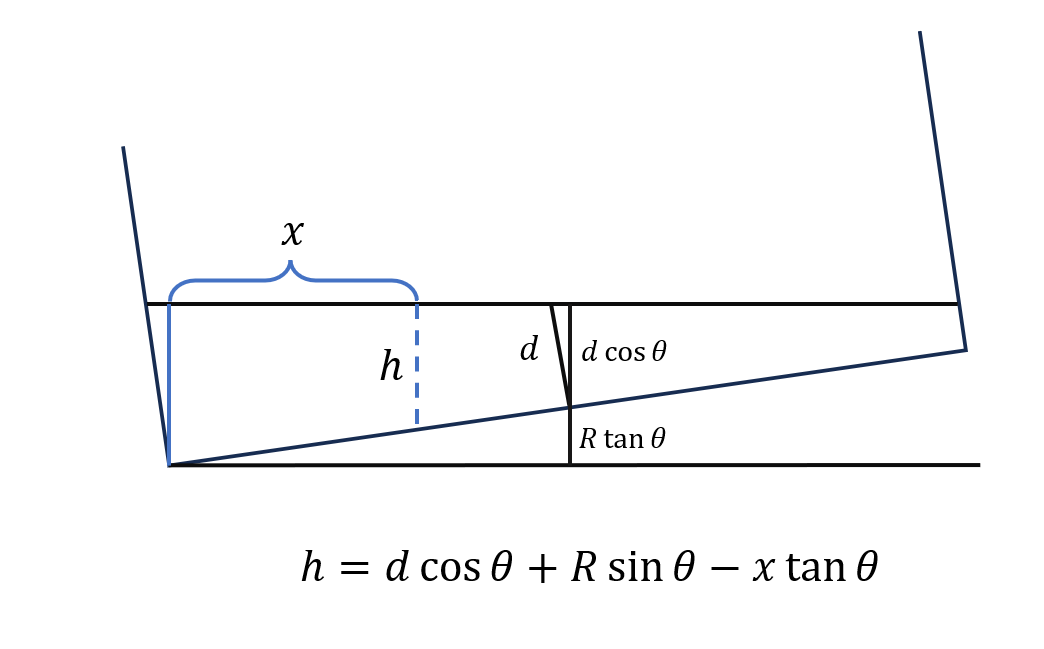
\includegraphics[width = 0.5\textwidth]{实验原理示意.png}
	\caption{厚度计算示意图}
\end{figure}
可见在小角度范围内，液膜厚度沿 $x$ 方向近似线性变化；倾斜角 $\theta$ 越大，厚度梯度越明显。因此固定体积 $V$、浓度 $c$ 与角度 $\theta$，即可由几何关系唯一确定液膜厚度分布，据此生成用于对比训练的深度图（具体程序见附录）。

\subsection{Beer-Lambert 定律与颜色映射}
蓝色染料对光的吸收满足 Beer-Lambert 定律
\[
	A = \lg (\frac{I_0}{I}) = Klc
\]
其中 $A$ 为吸光度，$I_0$ 为入射光强，$I$ 为透射光强，$l$ 为光程（此处即液膜厚度 $h$），$c$ 为染料浓度，$K$ 为吸收系数。液膜厚度不同，吸光度不同，透射光强也不同，最终体现在相机 CMOS 采样的 sRGB 值上。通过建立“特定光谱吸收—光强—图像像素深度（sRGB）”的映射模型，即可由图像颜色信息反演液膜厚度。

注意到，Beer-Lambert 定律反应了对应溶液在响应的波长的吸收，实际需要查阅数据，获取特定染料的吸收光谱，经过吸光度测算和sRGB通道的耦合，可以对特定的浓度给出对应像素的sRGB。使用这种算法同时对深度图进行对照，可以验证标定的有效性。

对于一个使用相机拍摄成像的系统，其核心是把光学信息经过模数转化，最终变为一个像素点的rgb值。对于这个系统，首先，白光涩味6500K，能获取对应的光谱，这个光谱经过了薄层染料的吸收，根据吸收光谱对应每一个波长值的吸收，获得吸收后的光谱和强度信息。这个光谱，经过相机采样，和gamma=2的修正，会映射到一张图像。因此厚度到一个sRGB坐标是单射。到rgb三通道的耦合相当于一个投影过程，所以逆过程是不可行的，也即无法通过sRGB回到光谱。可以通过正向过程生成模拟的颜色深度图，后期混合真实数据和模拟图像训练。比对模拟图和真实采样图，来衡量标注质量。

此处列举几组标注数据和实际数据，其中左侧三组为实际采样的图片，右侧一列为程序模拟图。
\begin{figure}[H]
	\centering
	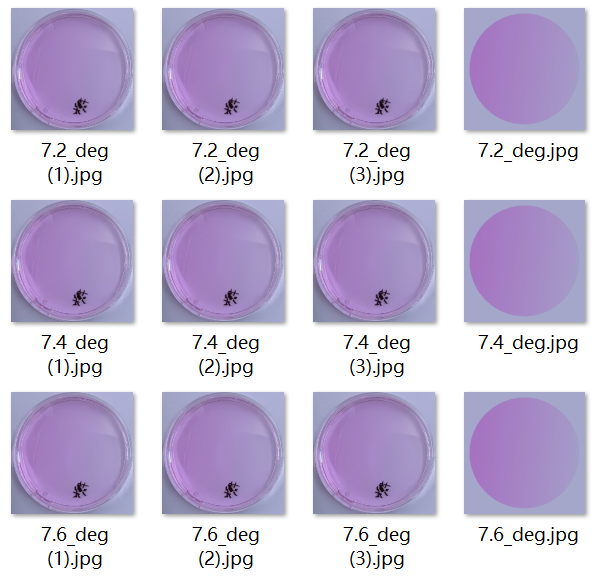
\includegraphics[width = 0.6\textwidth]{数据举例.png}
	\caption{实际采集数据和模拟数据比较}
\end{figure}
%此处插入CMOS采集亮度数据等内容，经过解析得到图像的过程，并给出逆过程。
该染料的一些吸收特性如下，考虑了实际在相机采样时的底色不一定完全是白色，在采集一些样本后，给出了一个基准值：
\begin{figure}[H]
	\centering
	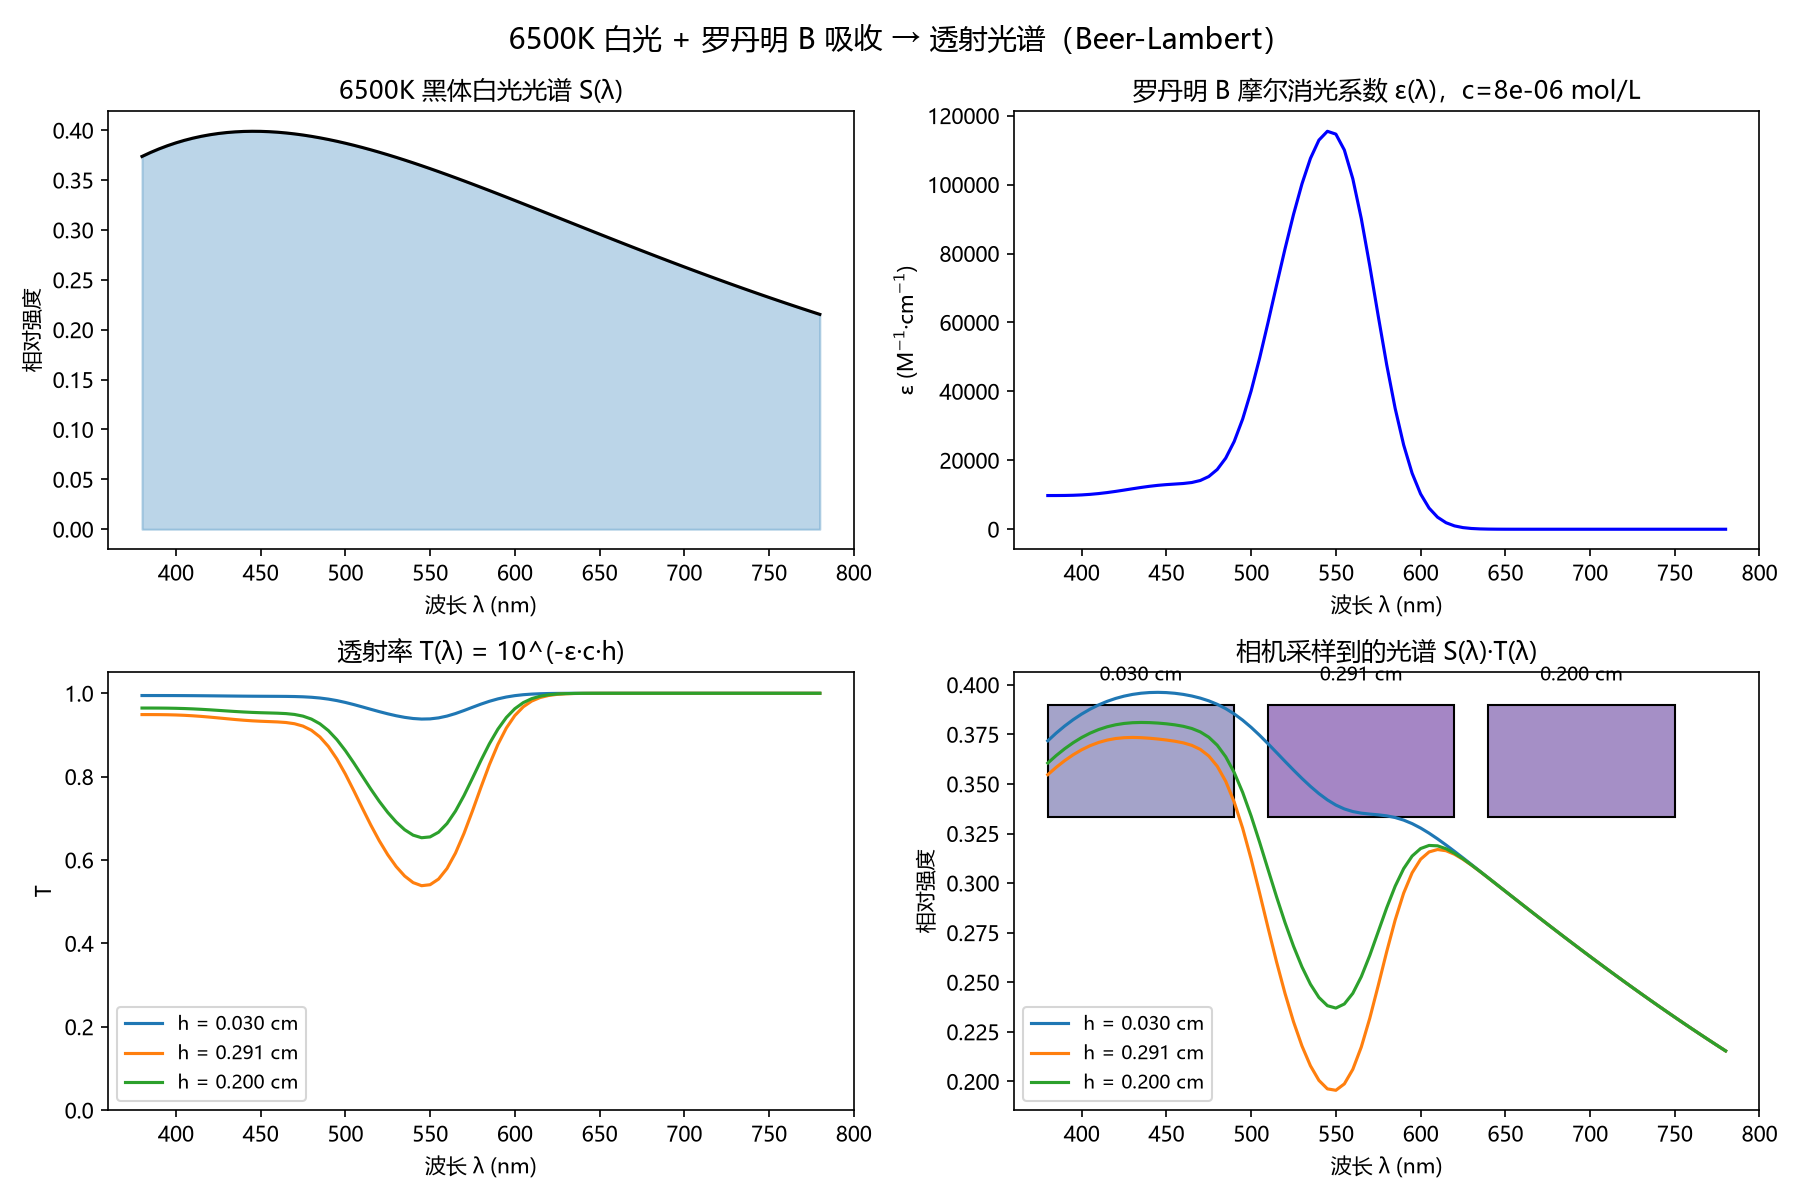
\includegraphics[width = 0.6\textwidth]{spectra_6500k_rhodamine.png}
	\caption{罗丹明染料的吸收特性}
	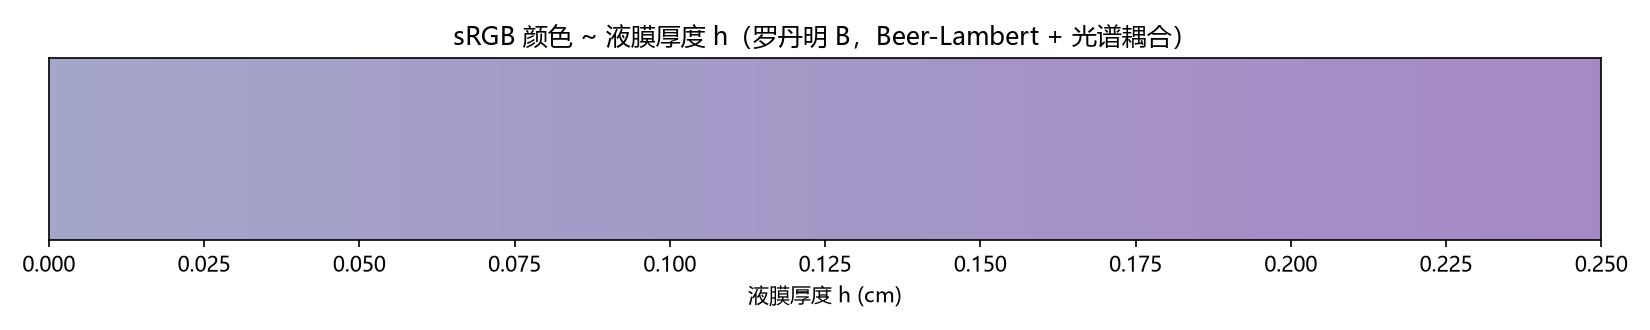
\includegraphics[width = 0.6\textwidth]{color_vs_thickness_rhodamine.png}
	\caption{罗丹明染料的浓度与采样颜色}
\end{figure}
如图，发现模拟产生的图像与实际采样的图像很类似，所以基本上可以认定标注数据的准确性。此处存在一个未来的研究方向：可以提出定量的方法衡量数据标注的质量。

\subsection{试图模拟的水膜厚度与颜色关系}
已知一个上下均为空气介质的水膜，如果有光从一侧摄入，光会在上下表面发生折反射，根据Fernel定律可以得到光的折反射率，外加位相变化，可以计算不同波长的光对应的光强。如图所示
\begin{figure}[H]
	\centering
	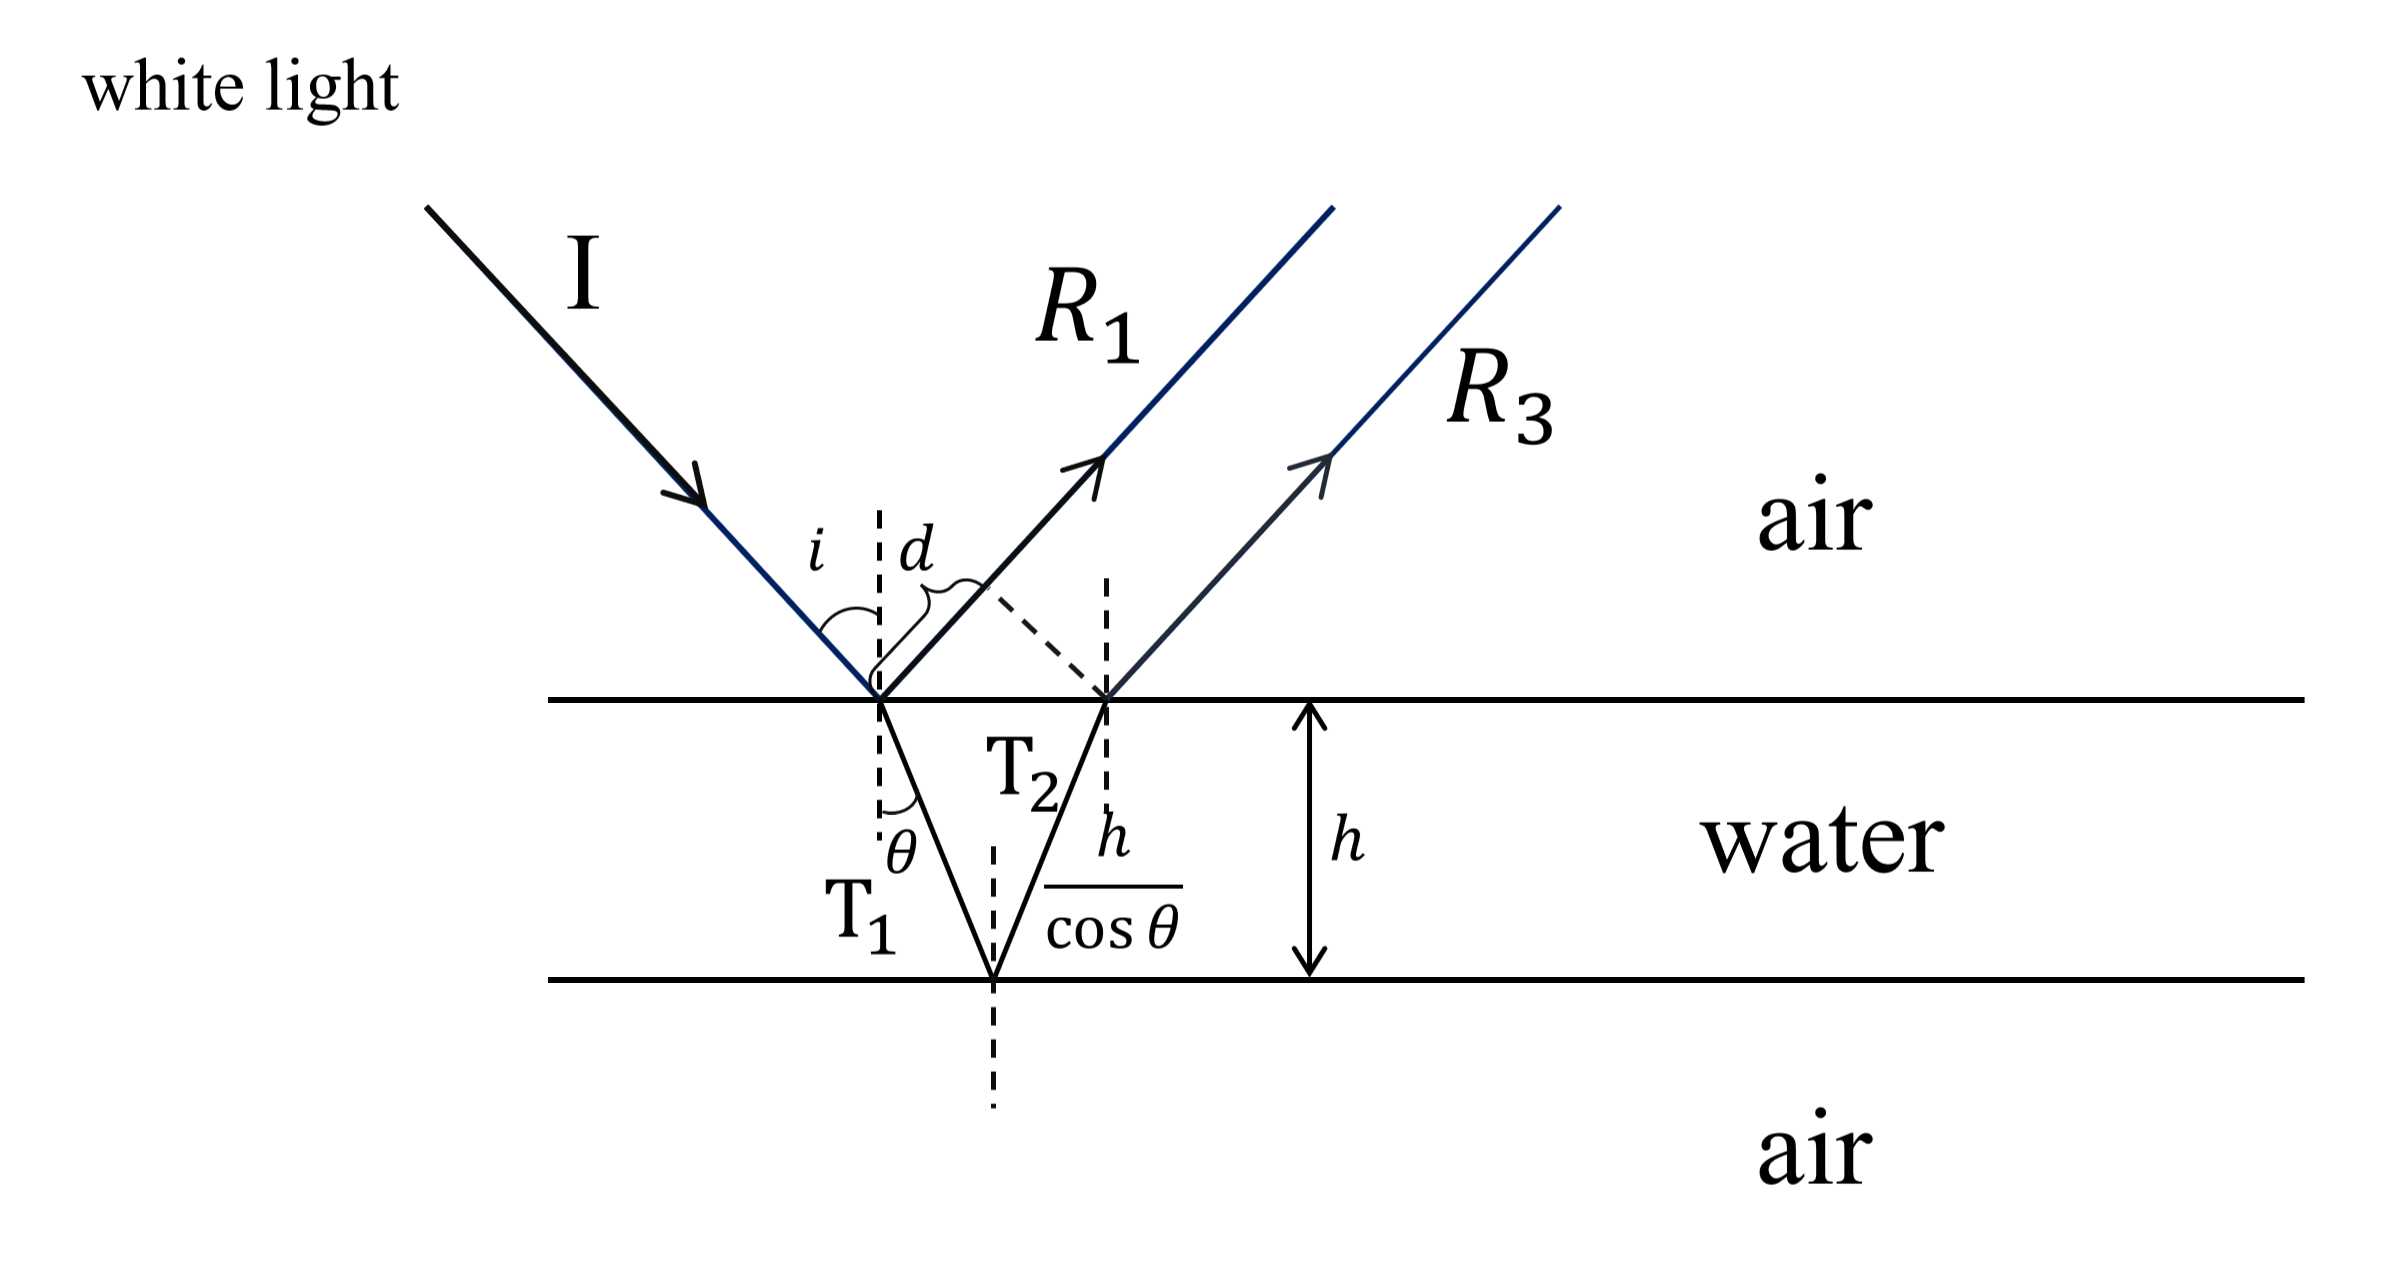
\includegraphics[width = 0.8\textwidth]{光学原理.png}
	\caption{薄膜两侧上下干涉示意图}
\end{figure}
入射光为$I$，在水膜表面第一次反射的反射光为$R_1$，折射光为$T_1$，下表面二次反射，反射光为$T_2$，再次通过水膜表面的光为$R_3$。首先计算$R_3$和$R_1$之间的光程差，其中水的折射率会随波长变化，此处用$n(\lambda)$表示，在不引起歧义时用n表示，另外空气的折射率定为1。由图可知，首先图中的$d = 2h\tan \theta \sin i$，又由\(n\sin \theta=\sin i\)因此光程差为
\[\Delta =2 n(\lambda) \frac h {\cos \theta}- 2h\tan \theta \sin i=2n(\lambda)h\cos \theta\]
位相差随即变为
\[\phi =\frac{4\pi n(\lambda)h\cos \theta}{\lambda}\]
图中画的是入射角为一般角度的情形，为了方便看清，实际上采用的是垂直入射$\theta=0^\circ$，此时s偏振和p偏振不做区分，此时使用菲涅尔公式以反馈反射光光强。
\[\frac{E_{R1}}{E_I}=\frac{1-n}{1+n}\]
\[\frac{E_{R3}}{E_I}=\frac{2}{1+n} \cdot \frac{n-1}{1+n} \cdot \frac{2n}{1+n}\]
注意到，这里自带了一个符号，已经加入了半波损失，于是光强可以这样表示
\[\tilde{U}=E_{R1}+E_{R3}\cdot e^{i\phi}\]
\[I =|\tilde{U}|^2 \]
不同波长的光会对应不同的光强，结合起来就会显示出不同颜色，将光在水中传播的衰减考虑进去后，通过程序计算模拟出的光谱如下：
\begin{figure}[H]
	\centering
	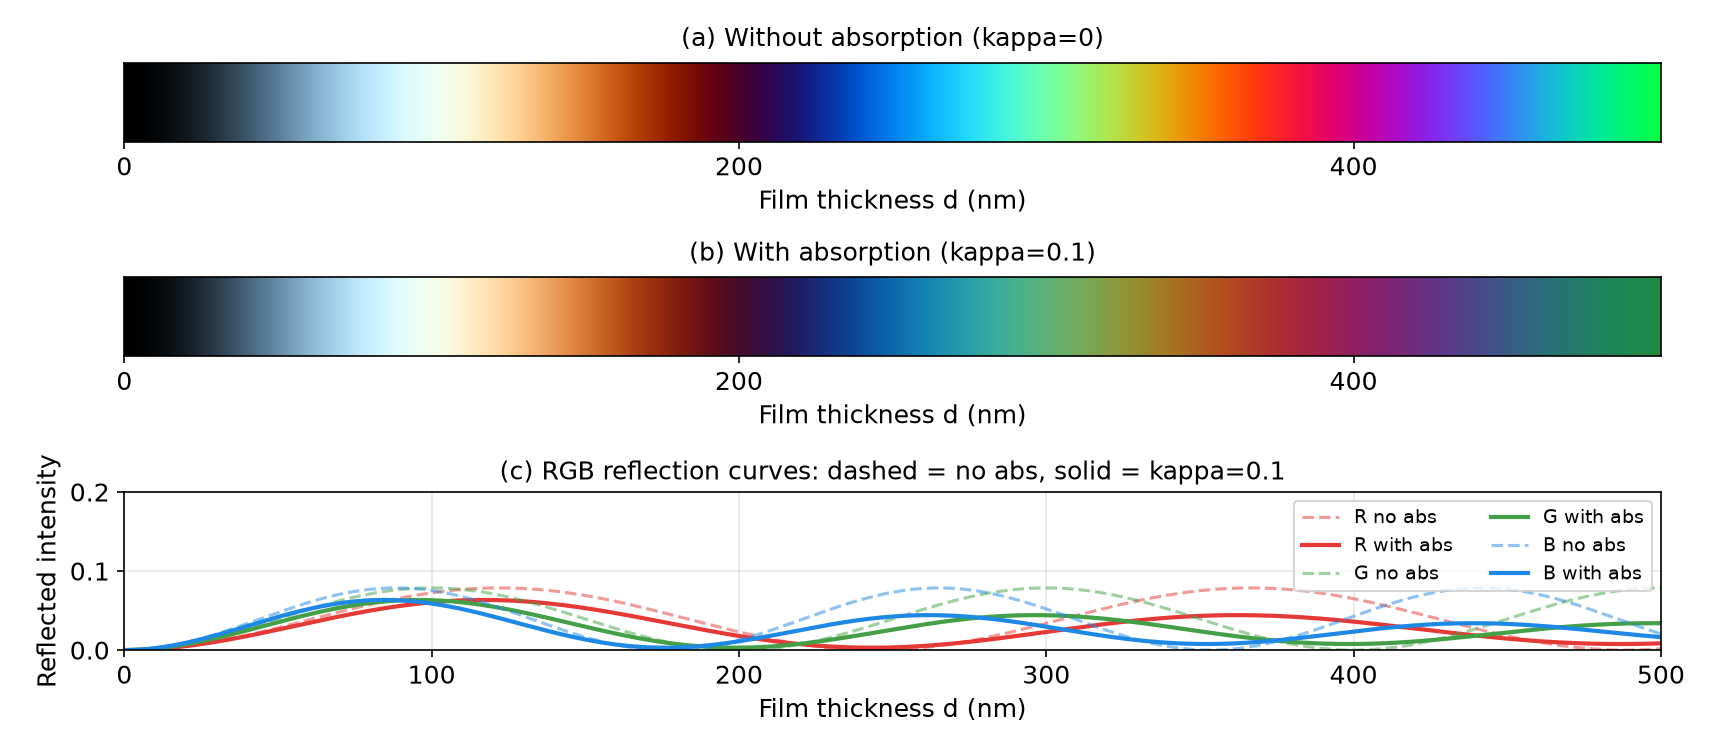
\includegraphics[width = 0.6\textwidth]{Figure_1.png}
	\caption{反射光颜色和厚度模拟图}
\end{figure}
注意到在膜很薄（<100nm）时，颜色是蓝黑色的，使用蓝色染料可以拟合出这种颜色的变化以此证明可以用机器学习的方法预测膜厚。本实验由于条件所限，只能使用罗丹明染料，同样可以对使用颜色判断厚度提供支撑。

\section{实验过程}
\subsection{装置搭建}
将 X 轴角度倾斜平台固定在光学工作平面上，顶部使用M4螺丝外接转接板，在倾斜平面上放置均匀白光光源（或平板，手机等发出白光的物件），光源上垫一张白纸以形成漫反射光并增大摩擦力（玻璃—纸张—玻璃不滑动），再于其上放置培养皿。在顶部固定相机或手机，调节镜头中心光轴与培养皿中心对齐，锁定焦距及各项参数；必要时用黑布或暗箱遮光以消除环境光。装置示意图如图~\ref{fig:setup} 所示。实际搭建过程中发现在培养皿底部放置白纸亦可以模拟出底部均匀光照的漫反射，无需额外增加发光底板。由于实验器材的某些原因，存在液面表面反射光干扰数据的情况，需要在数据处理时额外处理。

\begin{figure}[H]
	\centering
	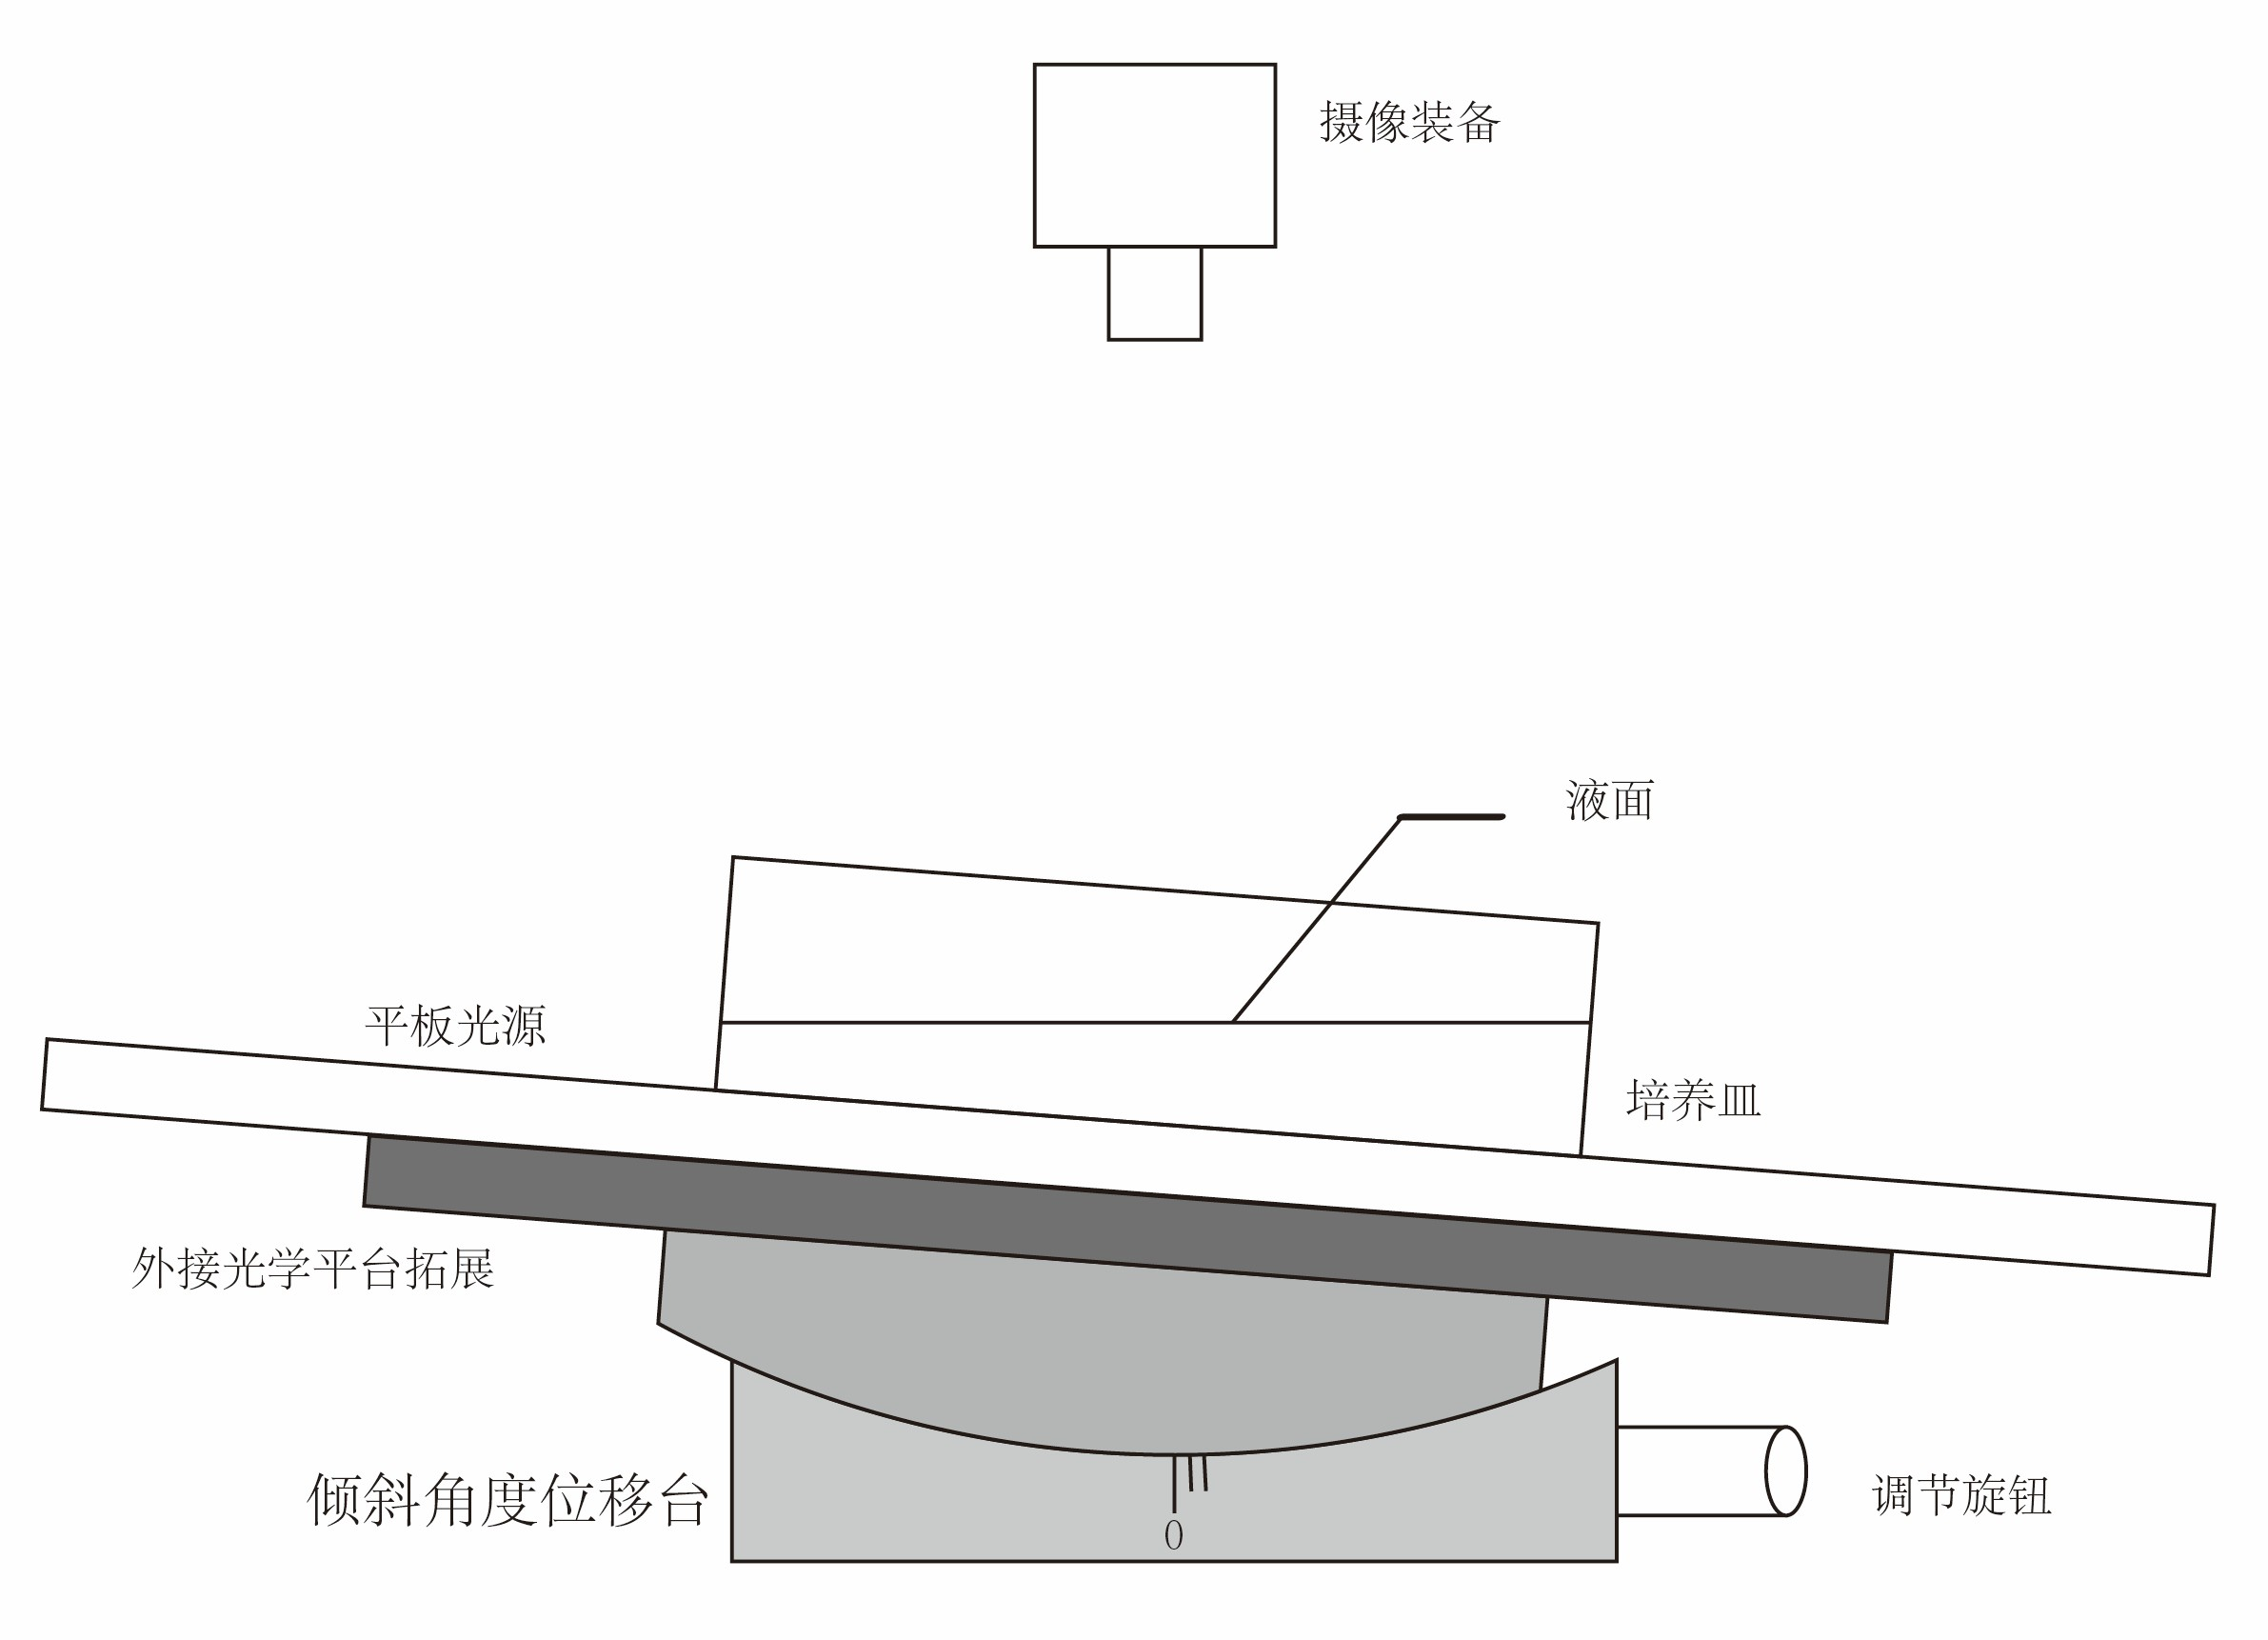
\includegraphics[width=0.6\textwidth]{实验装置图.jpg}
	\caption{液膜测厚实验装置示意图}
	\label{fig:setup}
\end{figure}
如果没有倾斜角度位移台，也可以考虑如下的方案，使用一个一维的x轴位移台，通过转接的方式，改造成z方向位移台，右侧使用一个垫高的滑块或者另一个一维位移台。此设计的不方便之处在于需要手动读取两个位移台的示数差以及两个位移台之间的距离，并且计算得到角度。如图~\ref{fig:set2}所示。
\begin{figure}[H]
	\centering
	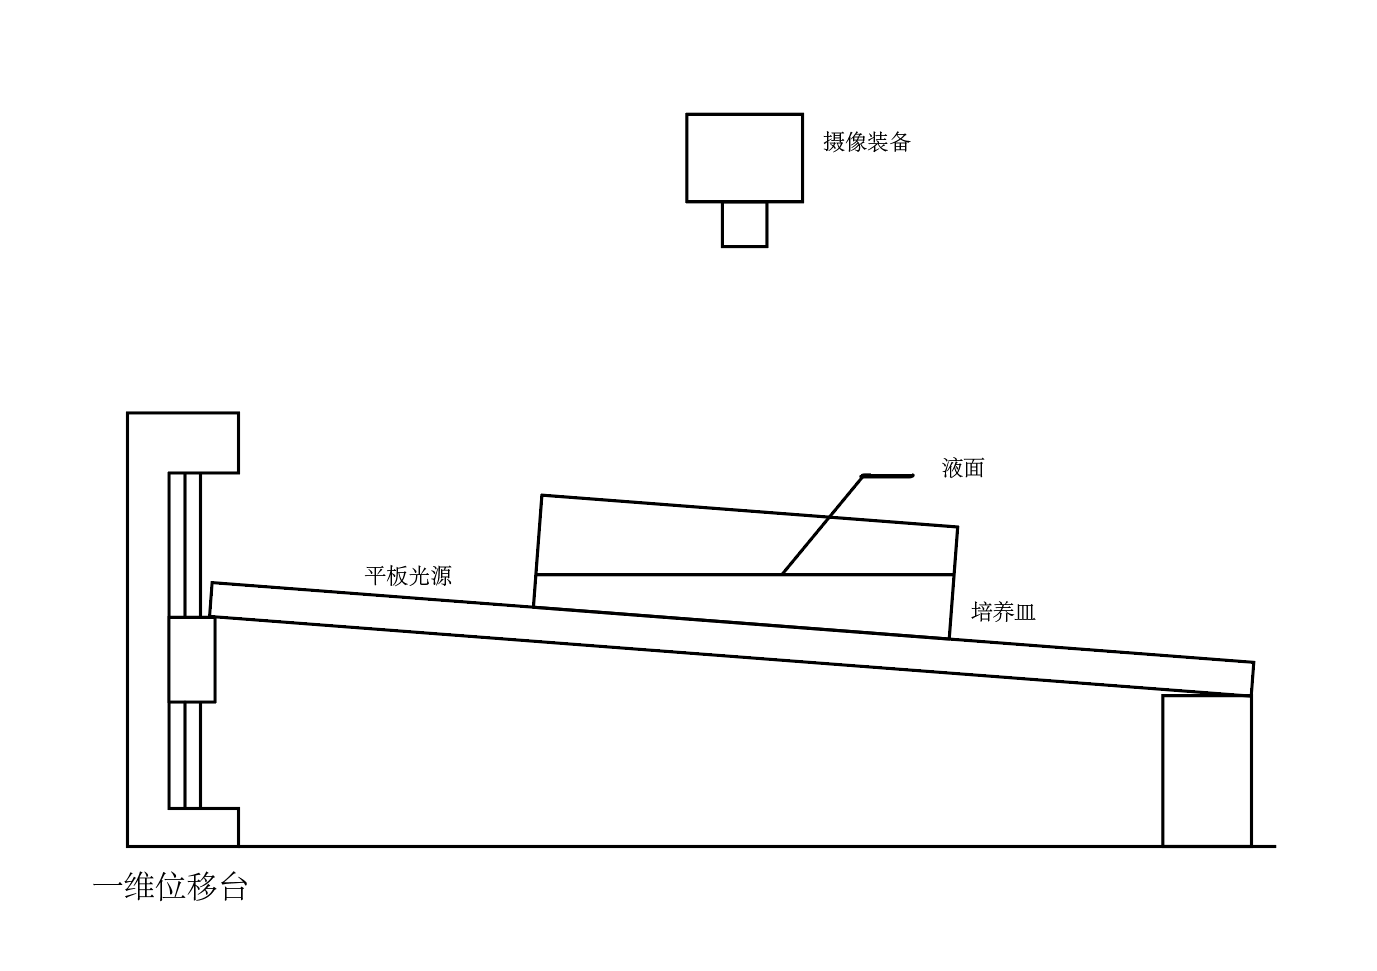
\includegraphics[width = 0.6\textwidth]{实验装置图2.png}
	\caption{使用z轴位移台的实验装置示意}
	\label{fig:set2}
\end{figure}
\subsection{参数测量}
用游标卡尺测量培养皿的深度、直径（$2R$）与底部厚度（$D$）；配制并注入固定体积 $V$、固定浓度 $c$ 的蓝色染液。实验种不能改变浓度，因为改变浓度和改变体积会达成同样的效果，需要控制变量；可以改变体积（需要重新使用程序生成对应体积的tiff图）。

实际拍摄参数：快门速度s=100；白平衡6500K，实际所用光源色温也是6500K；ISO： 250；f=2.2。倾斜轴与相机横向画面的轴夹角为6$^\circ$。

\subsection{图像采集}
固定相机参数后进行手动角度扫描：倾斜角从 $0^\circ$ 到 $9.6^\circ$，步长 $0.1^\circ$，共 97 个角度；每个角度采集 3 帧，共获取 291 张图像。采集完成后对白平衡等进行微调，图像左右镜像，以此进行数据增强，人为构造更大的样本集。

\subsection{数据处理与标注}
编写程序，依据几何模型解析生成每幅图像对应的液膜厚度（深度图），并使其与 RGB 图像对齐（后期通过程序对齐，或根据实验中设置的参考对齐）。将数据集按 72\% 训练、8\% 验证、20\% 测试划分；用 Beer-Lambert 拟合等简单模型检验标注质量，再用深度学习模型（U-Net 等）训练，实现由图像反演液膜厚度。

数据人为增强：调整图像的白平衡，不同颜色会有不同的现象。将图像进行多角度翻转，可以提升模型的鲁棒性。
\subsection{普通u-net模型}
设计流程如下：初始拍摄获取的图片为3120*3120pixel，对其进行压缩，压缩到384*384（由于u-net必须将样本划分为16份，所以这里的像素必须是16的整数倍，另外又需要控制训练的时间，所以选择这个尺寸进行压缩），使用u-net模型，将损失函数定义如下，对于每一个像素点的厚度，取其偏差值的平方，也就是所有有效像素的均方误差。为了方便运算，首先根据出现的厚度最大值和最小值，将实际输入的厚度值归一化到[0,1]之后再进行训练。

\[d_i=(d_{pred}-d_{target})^2\]

\[LOSS = \frac{\sum_{\text{有效像素}}d_i}{\text{有效像素数}} \]

基于这个损失函数，结合学习率$1\times 10^{-3}$的Adam优化器进行训练。以达到损失函数最小。另外，可以在损失函数中加入物理条件的限制。

\subsection{结合物理规律约束训练}
为了增强模型预测厚度与图像颜色之间的物理一致性，训练时引入了基于 Beer-Lambert 吸收与 sRGB 渲染的物理约束。具体地，将网络预测的厚度先反归一化为真实厚度，再通过 \texttt{absorbed.py} 中的光谱模型，计算对应的物理 sRGB 值；然后将渲染得到的 sRGB 与输入图像的真实 RGB 进行比较，构造一个额外的物理损失项。

该物理损失项与厚度均方误差损失共同构成最终训练目标：

\[LOSS = LOSS_{thickness} + \lambda \cdot LOSS_{physics},\]

其中 $LOSS_{physics}$ 为预测厚度生成的 sRGB 与真实图像 RGB 之间的像素级 L2 误差，权重 $\lambda$ 取值为 0.1。此约束促使模型不仅在厚度空间逼近真实值，而且在颜色空间满足物理吸收规律，从而减少厚度预测与实际光谱颜色之间的不一致性。

\section{实验结果}
\subsection{实验现象}
\begin{enumerate}
	\item 培养皿水平放置时，液面颜色均匀，不同区域无明显色差；
	\item 倾斜培养皿后，液膜呈楔形，液膜较厚（低端）处颜色明显加深，液膜较薄（高端）处颜色变浅，沿倾斜方向形成连续的颜色渐变；
	\item 倾斜角 $\theta$ 增大时，颜色渐变更加明显；同一角度下，颜色沿 $x$ 方向近似均匀、线性变化；
	\item 注意到由于玻璃表面不是完全亲水的，在培养皿周围存在着因表面张力引起的液膜弯曲，一定程度上影响线性假设。液面表面也有来自顶部照射光源的反射光，且反射情况随着液面角度变化有所变化，在实际训练时需要调整。
	\item 改变光源亮度或白平衡后，图像整体明暗与色调随之变化，说明颜色对光源与相机参数较为敏感，采集时需锁定参数。
\end{enumerate}

\subsection{数据记录}
培养皿及溶液参数如表~\ref{tab:para} 所示。
\begin{table}[H]
	\centering
	\caption{培养皿与溶液参数}
	\label{tab:para}
	\begin{tabular}{lc}
		\toprule
		参数 & 数值 \\ \midrule
		培养皿直径 $2R$ (mm) & 31.72 \\
		培养皿深度 (mm) & 4.62 \\
		培养皿底部厚度 $D$ (mm) & 1.14 \\
		染液体积 $V$ (mL) & 2.3 \\
		染液平坦厚度 $d$(mm) & 2.91\\
		染液名称 & 罗丹明 \\
		染料浓度 $c$(mol/L) & $1\times 10^{-5}$ \\
		采集角度范围 ($^\circ$) & 0 -- 9.6，步长 0.1 \\
		每角度帧数 & 3 \\
		总图像数 (张) & 291\\
		训练/验证/测试图像数 (张) & 210 / 24 / 57 \\
		\bottomrule
	\end{tabular}
\end{table}

u-net模型训练与评估结果见表~\ref{tab:model}。
\begin{table}[H]
	\centering
	\caption{模型训练与评估结果}
	\label{tab:model}
	\begin{tabular}{lc}
		\toprule
		项目 & 数值 \\ \midrule
		验证集最优 RMSE & $0.0949\ \mathrm{mm}$ \\
		验证集最优 MAE & $0.0567\ \mathrm{mm}$ \\
		测试集 RMSE & $0.0947\ \mathrm{mm}$ \\
		测试集 MAE & $0.0523\ \mathrm{mm}$ \\
		厚度反演相对误差 & 1.80\%\\
		\bottomrule
	\end{tabular}
\end{table}

添加了物理约束的模型训练评估结果如下：
\begin{table}[H]
	\centering
	\caption{物理约束模型训练与评估结果}
	\begin{tabular}{lc}
		\toprule
		项目 & 数值 \\ \midrule
		验证集最优 RMSE & $0.0901\ \mathrm{mm}$ \\
		验证集最优 MAE & $0.0525\ \mathrm{mm}$ \\
		测试集 RMSE & $0.0929\ \mathrm{mm}$ \\
		测试集 MAE & $0.0517\ \mathrm{mm}$ \\
		物理约束损失权重 $\lambda$ & $0.1$ \\
		\bottomrule
	\end{tabular}
\end{table}
从各方面评估，物理约束的模型准确度更高。
训练中给出的预测图比对如下：
\begin{figure}[H]
	\centering
	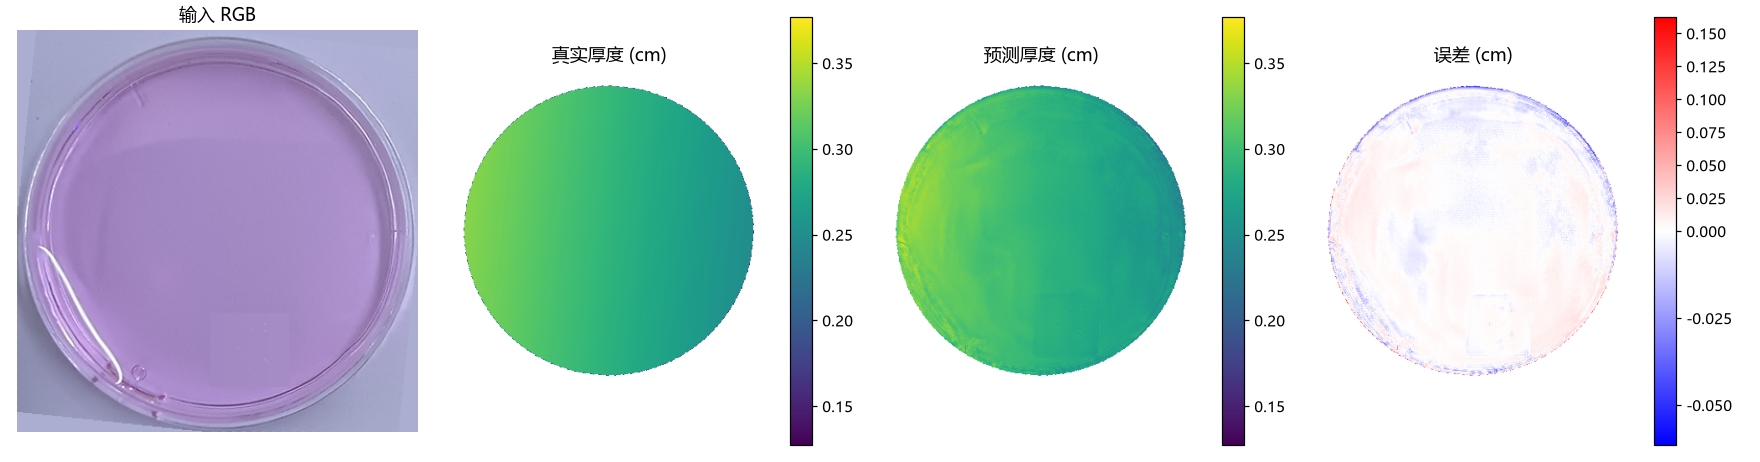
\includegraphics[width = 0.6\textwidth]{pred_1.5_deg (3)_compare.png}
	\caption{1.5度角预测}
\end{figure}
\begin{figure}[H]
	\centering
	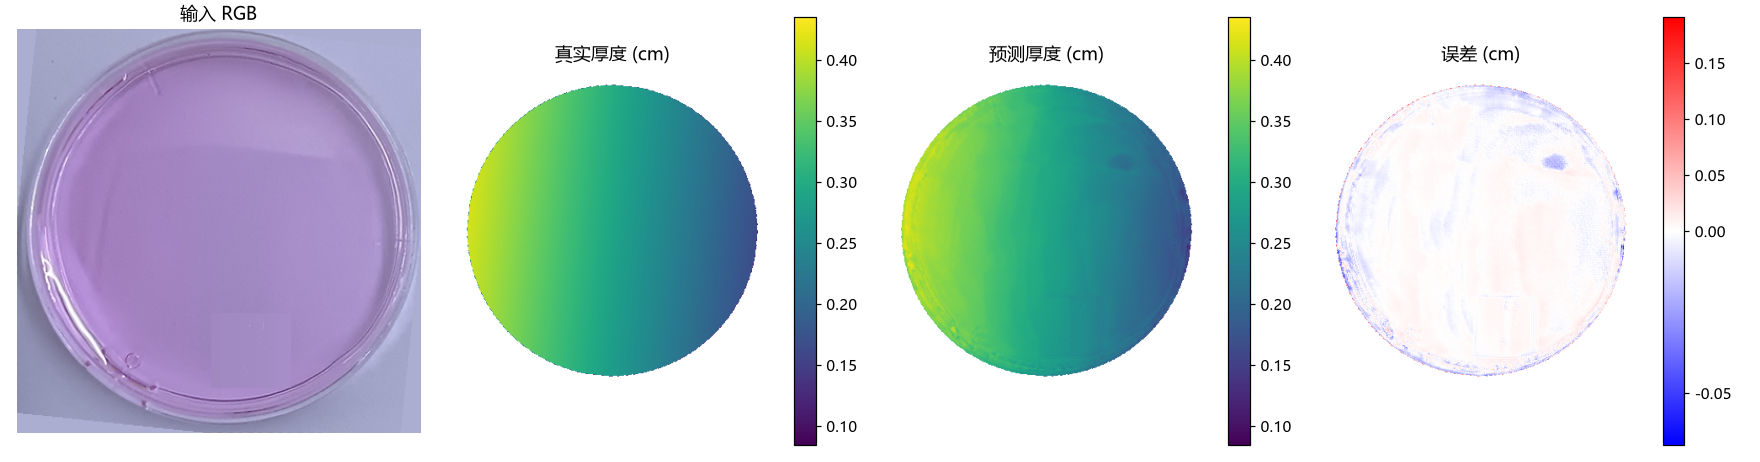
\includegraphics[width = 0.6\textwidth]{pred_4.5_deg (3)_compare.png}
	\caption{4.5度角预测}
\end{figure}
\begin{figure}[H]
	\centering
	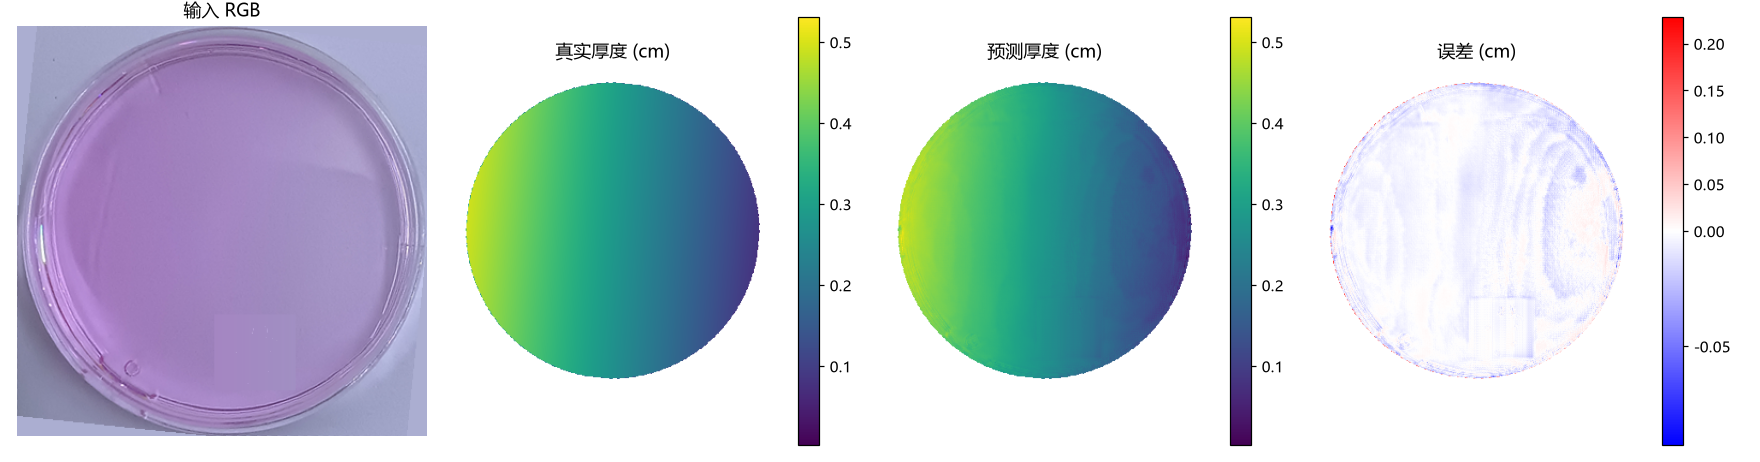
\includegraphics[width = 0.6\textwidth]{pred_7.5_deg (3)_compare.png}
	\caption{7.5度角预测}
\end{figure}
\section{结论}
本实验搭建了“倾斜位移台—均匀漫射光源—相机”的液膜测厚图像采集系统，通过倾斜培养皿使液膜厚度沿水平方向线性变化，并依据 Beer-Lambert 定律建立了液膜厚度与颜色（吸光度）之间的定量关系。实验现象表明，液膜颜色随厚度增大而明显加深，厚度与颜色存在稳定的对应关系。基于采集的数据集训练深度学习模型后，模型能够由单幅图像反演液膜厚度分布；在测试集上，厚度反演误差约为 0.0523 mm，相对误差约为 1.80\%，与几何模型给出的理论厚度符合较好。在误差允许的范围内，验证了基于颜色信息测量液体厚度的可行性。

\textbf{未来研究方向：}
\begin{enumerate}
	\item 更换光源、更改白平衡或相机种类进一步检验模型的泛化能力
	\item 采集更多数据以提升反演精度
	\item 改进物理规律的约束方式
	\item 设计定量刻画数据标注质量的方法
	\item 标注数据与训练样本的对齐操作
	
\end{enumerate}

本实验试图模拟水膜在极薄时可能出现的蓝黑色，通过验证用颜色预测深度的可行性，以此论证在薄液膜测厚上机器学习算法的应用。所用代码参见相关文件。
\end{document}